% Options for packages loaded elsewhere
\PassOptionsToPackage{unicode}{hyperref}
\PassOptionsToPackage{hyphens}{url}
\documentclass[
  11pt,
]{article}
\usepackage{xcolor}
\usepackage[margin=1in]{geometry}
\usepackage{amsmath,amssymb}
\setcounter{secnumdepth}{5}
\usepackage{iftex}
\ifPDFTeX
  \usepackage[T1]{fontenc}
  \usepackage[utf8]{inputenc}
  \usepackage{textcomp} % provide euro and other symbols
\else % if luatex or xetex
  \usepackage{unicode-math} % this also loads fontspec
  \defaultfontfeatures{Scale=MatchLowercase}
  \defaultfontfeatures[\rmfamily]{Ligatures=TeX,Scale=1}
\fi
\usepackage{lmodern}
\ifPDFTeX\else
  % xetex/luatex font selection
\fi
% Use upquote if available, for straight quotes in verbatim environments
\IfFileExists{upquote.sty}{\usepackage{upquote}}{}
\IfFileExists{microtype.sty}{% use microtype if available
  \usepackage[]{microtype}
  \UseMicrotypeSet[protrusion]{basicmath} % disable protrusion for tt fonts
}{}
\makeatletter
\@ifundefined{KOMAClassName}{% if non-KOMA class
  \IfFileExists{parskip.sty}{%
    \usepackage{parskip}
  }{% else
    \setlength{\parindent}{0pt}
    \setlength{\parskip}{6pt plus 2pt minus 1pt}}
}{% if KOMA class
  \KOMAoptions{parskip=half}}
\makeatother
\usepackage{color}
\usepackage{fancyvrb}
\newcommand{\VerbBar}{|}
\newcommand{\VERB}{\Verb[commandchars=\\\{\}]}
\DefineVerbatimEnvironment{Highlighting}{Verbatim}{commandchars=\\\{\}}
% Add ',fontsize=\small' for more characters per line
\usepackage{framed}
\definecolor{shadecolor}{RGB}{248,248,248}
\newenvironment{Shaded}{\begin{snugshade}}{\end{snugshade}}
\newcommand{\AlertTok}[1]{\textcolor[rgb]{0.94,0.16,0.16}{#1}}
\newcommand{\AnnotationTok}[1]{\textcolor[rgb]{0.56,0.35,0.01}{\textbf{\textit{#1}}}}
\newcommand{\AttributeTok}[1]{\textcolor[rgb]{0.13,0.29,0.53}{#1}}
\newcommand{\BaseNTok}[1]{\textcolor[rgb]{0.00,0.00,0.81}{#1}}
\newcommand{\BuiltInTok}[1]{#1}
\newcommand{\CharTok}[1]{\textcolor[rgb]{0.31,0.60,0.02}{#1}}
\newcommand{\CommentTok}[1]{\textcolor[rgb]{0.56,0.35,0.01}{\textit{#1}}}
\newcommand{\CommentVarTok}[1]{\textcolor[rgb]{0.56,0.35,0.01}{\textbf{\textit{#1}}}}
\newcommand{\ConstantTok}[1]{\textcolor[rgb]{0.56,0.35,0.01}{#1}}
\newcommand{\ControlFlowTok}[1]{\textcolor[rgb]{0.13,0.29,0.53}{\textbf{#1}}}
\newcommand{\DataTypeTok}[1]{\textcolor[rgb]{0.13,0.29,0.53}{#1}}
\newcommand{\DecValTok}[1]{\textcolor[rgb]{0.00,0.00,0.81}{#1}}
\newcommand{\DocumentationTok}[1]{\textcolor[rgb]{0.56,0.35,0.01}{\textbf{\textit{#1}}}}
\newcommand{\ErrorTok}[1]{\textcolor[rgb]{0.64,0.00,0.00}{\textbf{#1}}}
\newcommand{\ExtensionTok}[1]{#1}
\newcommand{\FloatTok}[1]{\textcolor[rgb]{0.00,0.00,0.81}{#1}}
\newcommand{\FunctionTok}[1]{\textcolor[rgb]{0.13,0.29,0.53}{\textbf{#1}}}
\newcommand{\ImportTok}[1]{#1}
\newcommand{\InformationTok}[1]{\textcolor[rgb]{0.56,0.35,0.01}{\textbf{\textit{#1}}}}
\newcommand{\KeywordTok}[1]{\textcolor[rgb]{0.13,0.29,0.53}{\textbf{#1}}}
\newcommand{\NormalTok}[1]{#1}
\newcommand{\OperatorTok}[1]{\textcolor[rgb]{0.81,0.36,0.00}{\textbf{#1}}}
\newcommand{\OtherTok}[1]{\textcolor[rgb]{0.56,0.35,0.01}{#1}}
\newcommand{\PreprocessorTok}[1]{\textcolor[rgb]{0.56,0.35,0.01}{\textit{#1}}}
\newcommand{\RegionMarkerTok}[1]{#1}
\newcommand{\SpecialCharTok}[1]{\textcolor[rgb]{0.81,0.36,0.00}{\textbf{#1}}}
\newcommand{\SpecialStringTok}[1]{\textcolor[rgb]{0.31,0.60,0.02}{#1}}
\newcommand{\StringTok}[1]{\textcolor[rgb]{0.31,0.60,0.02}{#1}}
\newcommand{\VariableTok}[1]{\textcolor[rgb]{0.00,0.00,0.00}{#1}}
\newcommand{\VerbatimStringTok}[1]{\textcolor[rgb]{0.31,0.60,0.02}{#1}}
\newcommand{\WarningTok}[1]{\textcolor[rgb]{0.56,0.35,0.01}{\textbf{\textit{#1}}}}
\usepackage{longtable,booktabs,array}
\newcounter{none} % for unnumbered tables
\usepackage{calc} % for calculating minipage widths
% Correct order of tables after \paragraph or \subparagraph
\usepackage{etoolbox}
\makeatletter
\patchcmd\longtable{\par}{\if@noskipsec\mbox{}\fi\par}{}{}
\makeatother
% Allow footnotes in longtable head/foot
\IfFileExists{footnotehyper.sty}{\usepackage{footnotehyper}}{\usepackage{footnote}}
\makesavenoteenv{longtable}
\usepackage{graphicx}
\makeatletter
\newsavebox\pandoc@box
\newcommand*\pandocbounded[1]{% scales image to fit in text height/width
  \sbox\pandoc@box{#1}%
  \Gscale@div\@tempa{\textheight}{\dimexpr\ht\pandoc@box+\dp\pandoc@box\relax}%
  \Gscale@div\@tempb{\linewidth}{\wd\pandoc@box}%
  \ifdim\@tempb\p@<\@tempa\p@\let\@tempa\@tempb\fi% select the smaller of both
  \ifdim\@tempa\p@<\p@\scalebox{\@tempa}{\usebox\pandoc@box}%
  \else\usebox{\pandoc@box}%
  \fi%
}
% Set default figure placement to htbp
\def\fps@figure{htbp}
\makeatother
\setlength{\emergencystretch}{3em} % prevent overfull lines
\providecommand{\tightlist}{%
  \setlength{\itemsep}{0pt}\setlength{\parskip}{0pt}}
\usepackage{amsmath}
% Shared LaTeX preamble for all Data Mining / ISLR chapter documents.
% Provides \makecoverpage{<assignment title>} — a standalone title page
% with fixed student identity, so every chapter/lab looks uniform.

\usepackage{graphicx}

\newcommand{\makecoverpage}[1]{%
\begin{titlepage}
\centering
\vspace*{2cm}

{\Large \textbf{Adventist University of Central Africa}}\\[0.4cm]
{\large Master's in Big Data Analytics}\\[2cm]

{\Huge \textbf{#1}}\\[0.5cm]
{\large \textit{Introduction to Statistical Learning with Applications in R}}\\[3cm]

\begin{tabular}{rl}
\textbf{Programme:} & MSc Big Data Analytics \\
\textbf{Course Title:} & Data Mining \\
\textbf{Course Code:} & MSDA 9124 \\
\textbf{Lecturer:} & Dr. Pacifique Nizeyimana \\
\textbf{Student Name:} & Wayne Rubangisa \\
\textbf{Student ID:} & 101220 \\
\end{tabular}

\vfill

{\large September 2026}

\end{titlepage}
}

\usepackage{bookmark}
\IfFileExists{xurl.sty}{\usepackage{xurl}}{} % add URL line breaks if available
\urlstyle{same}
\hypersetup{
  hidelinks,
  pdfcreator={LaTeX via pandoc}}

\author{}
\date{\vspace{-2.5em}}

\begin{document}

\makecoverpage{Chapter 5 --- Resampling Methods \\ Lab}

\section{Introduction}\label{introduction}

When a model is fitted, its training error is usually too optimistic:
the same observations were used both to estimate the model and to
measure how well it fits. The real questions are different. How well
will the model predict new observations? How much would its coefficients
change if we had collected a different sample? Which model complexity
gives the best balance between underfitting and overfitting?

Resampling methods answer these questions by repeatedly reusing the
observed data in carefully chosen ways. This lab develops four closely
related ideas:

\begin{enumerate}
\def\labelenumi{\arabic{enumi}.}
\tightlist
\item
  the validation-set approach;
\item
  leave-one-out cross-validation (LOOCV);
\item
  \(k\)-fold cross-validation; and
\item
  the bootstrap.
\end{enumerate}

The first three estimate prediction error. The bootstrap estimates the
sampling variability of statistics such as regression coefficients and
portfolio weights. We use the \texttt{Auto} and \texttt{Portfolio} data
sets from \texttt{ISLR2}. The main prediction problem is to model
automobile fuel efficiency (\texttt{mpg}) from horsepower using
polynomial regression.

\begin{Shaded}
\begin{Highlighting}[]
\FunctionTok{library}\NormalTok{(ISLR2)}
\FunctionTok{library}\NormalTok{(boot)}
\end{Highlighting}
\end{Shaded}

\subsection{The prediction problem and the bias--variance
trade-off}\label{the-prediction-problem-and-the-biasvariance-trade-off}

Let \(Y\) be a response and \(X\) a predictor. A fitted model produces
\(\hat{f}(X)\), and its prediction error on a new observation can be
written as

\[
\mathbb{E}\left[(Y - \hat{f}(X))^2 \mid X=x\right]
= \underbrace{\sigma^2}_{\text{irreducible noise}}
+ \underbrace{\operatorname{Bias}\left[\hat{f}(x)\right]^2}_{\text{systematic error}}
+ \underbrace{\operatorname{Var}\left[\hat{f}(x)\right]}_{\text{sensitivity to the sample}}.
\]

A very simple model may have high bias because it cannot represent the
true relationship. A highly flexible model may have low training error
but high variance because it follows random details of the particular
sample. The purpose of resampling is to estimate the out-of-sample part
of this trade-off using only the data we have.

\section{Validation Set Approach}\label{validation-set-approach}

\subsection{Idea and mathematical
definition}\label{idea-and-mathematical-definition}

The validation-set approach randomly divides the data into a training
set and a validation set. We fit the model using only the training
observations, then evaluate predictions on observations that were not
used for fitting. For regression, the estimate is the validation mean
squared error (MSE):

\[
\operatorname{MSE}_{\mathrm{val}}
= \frac{1}{n_{\mathrm{val}}}
\sum_{i \in \mathcal{V}}
\left(y_i - \hat{f}_{\mathcal{T}}(x_i)\right)^2,
\]

where \(\mathcal{T}\) is the training set and \(\mathcal{V}\) is the
validation set. The notation on \(\hat{f}_{\mathcal{T}}\) matters: the
model was fitted using the training observations only.

The approach is easy and fast, but the result depends on one random
split. Also, because the model is trained on fewer observations than are
ultimately available, its validation error can be a little pessimistic.

\subsection{One training/validation
split}\label{one-trainingvalidation-split}

\texttt{Auto} contains 392 cars after missing observations have been
removed. We compare polynomial models of degrees one, two, and three. A
fixed seed makes the random split reproducible for the report.

\begin{Shaded}
\begin{Highlighting}[]
\FunctionTok{data}\NormalTok{(Auto)}
\NormalTok{Auto }\OtherTok{\textless{}{-}} \FunctionTok{na.omit}\NormalTok{(Auto)}
\NormalTok{n }\OtherTok{\textless{}{-}} \FunctionTok{nrow}\NormalTok{(Auto)}

\FunctionTok{set.seed}\NormalTok{(}\DecValTok{1}\NormalTok{)}
\NormalTok{train }\OtherTok{\textless{}{-}} \FunctionTok{sample}\NormalTok{(}\FunctionTok{seq\_len}\NormalTok{(n), }\AttributeTok{size =}\NormalTok{ n }\SpecialCharTok{/} \DecValTok{2}\NormalTok{)}
\NormalTok{validation }\OtherTok{\textless{}{-}} \SpecialCharTok{{-}}\NormalTok{train}

\NormalTok{validation\_mse }\OtherTok{\textless{}{-}} \ControlFlowTok{function}\NormalTok{(model, data, validation\_indices) \{}
  \FunctionTok{mean}\NormalTok{((data}\SpecialCharTok{$}\NormalTok{mpg }\SpecialCharTok{{-}} \FunctionTok{predict}\NormalTok{(model, }\AttributeTok{newdata =}\NormalTok{ data))[validation\_indices]}\SpecialCharTok{\^{}}\DecValTok{2}\NormalTok{)}
\NormalTok{\}}

\NormalTok{validation\_results }\OtherTok{\textless{}{-}} \FunctionTok{data.frame}\NormalTok{(}
  \AttributeTok{Degree =} \DecValTok{1}\SpecialCharTok{:}\DecValTok{3}\NormalTok{,}
  \AttributeTok{Validation\_MSE =} \FunctionTok{c}\NormalTok{(}
    \FunctionTok{validation\_mse}\NormalTok{(}\FunctionTok{lm}\NormalTok{(mpg }\SpecialCharTok{\textasciitilde{}}\NormalTok{ horsepower, }\AttributeTok{data =}\NormalTok{ Auto, }\AttributeTok{subset =}\NormalTok{ train), Auto, validation),}
    \FunctionTok{validation\_mse}\NormalTok{(}\FunctionTok{lm}\NormalTok{(mpg }\SpecialCharTok{\textasciitilde{}} \FunctionTok{poly}\NormalTok{(horsepower, }\DecValTok{2}\NormalTok{), }\AttributeTok{data =}\NormalTok{ Auto, }\AttributeTok{subset =}\NormalTok{ train), Auto, validation),}
    \FunctionTok{validation\_mse}\NormalTok{(}\FunctionTok{lm}\NormalTok{(mpg }\SpecialCharTok{\textasciitilde{}} \FunctionTok{poly}\NormalTok{(horsepower, }\DecValTok{3}\NormalTok{), }\AttributeTok{data =}\NormalTok{ Auto, }\AttributeTok{subset =}\NormalTok{ train), Auto, validation)}
\NormalTok{  )}
\NormalTok{)}
\NormalTok{validation\_results}
\end{Highlighting}
\end{Shaded}

\begin{verbatim}
##   Degree Validation_MSE
## 1      1       23.26601
## 2      2       18.71646
## 3      3       18.79401
\end{verbatim}

The model with the smallest validation MSE is preferred for this split.
The quadratic model normally improves substantially over the linear
model because fuel efficiency falls quickly at first and then levels
off. If the cubic model is not better, that is evidence that its extra
flexibility is fitting sample-specific variation rather than a reliable
pattern.

\begin{Shaded}
\begin{Highlighting}[]
\FunctionTok{plot}\NormalTok{(}
\NormalTok{  validation\_results}\SpecialCharTok{$}\NormalTok{Degree,}
\NormalTok{  validation\_results}\SpecialCharTok{$}\NormalTok{Validation\_MSE,}
  \AttributeTok{type =} \StringTok{"b"}\NormalTok{, }\AttributeTok{pch =} \DecValTok{19}\NormalTok{, }\AttributeTok{col =} \StringTok{"steelblue"}\NormalTok{,}
  \AttributeTok{xlab =} \StringTok{"Polynomial degree"}\NormalTok{, }\AttributeTok{ylab =} \StringTok{"Validation MSE"}\NormalTok{,}
  \AttributeTok{main =} \StringTok{"Validation error for polynomial models"}
\NormalTok{)}
\end{Highlighting}
\end{Shaded}

\begin{center}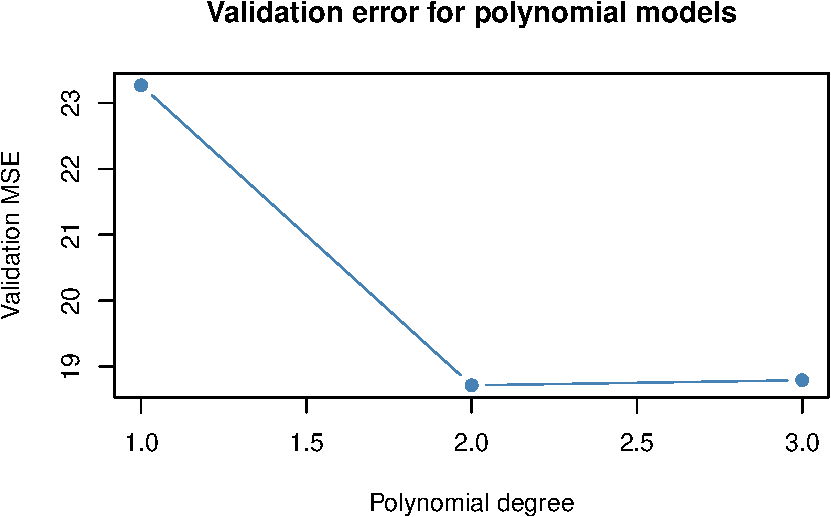
\includegraphics{ch05_lab_files/figure-latex/validation-plot-1} \end{center}

\subsection{Why one split is not
enough}\label{why-one-split-is-not-enough}

The validation set is itself a random sample. Changing the split changes
both the fitted coefficients and the observations used to judge them.
The model comparison is therefore noisy even when the underlying
data-generating process has not changed.

\begin{Shaded}
\begin{Highlighting}[]
\NormalTok{validation\_mse\_for\_seed }\OtherTok{\textless{}{-}} \ControlFlowTok{function}\NormalTok{(seed, degree) \{}
  \FunctionTok{set.seed}\NormalTok{(seed)}
\NormalTok{  training\_indices }\OtherTok{\textless{}{-}} \FunctionTok{sample}\NormalTok{(}\FunctionTok{seq\_len}\NormalTok{(n), }\AttributeTok{size =}\NormalTok{ n }\SpecialCharTok{/} \DecValTok{2}\NormalTok{)}
\NormalTok{  model\_formula }\OtherTok{\textless{}{-}} \ControlFlowTok{if}\NormalTok{ (degree }\SpecialCharTok{==} \DecValTok{1}\NormalTok{) \{}
\NormalTok{    mpg }\SpecialCharTok{\textasciitilde{}}\NormalTok{ horsepower}
\NormalTok{  \} }\ControlFlowTok{else}\NormalTok{ \{}
\NormalTok{    mpg }\SpecialCharTok{\textasciitilde{}} \FunctionTok{poly}\NormalTok{(horsepower, degree)}
\NormalTok{  \}}
\NormalTok{  model }\OtherTok{\textless{}{-}} \FunctionTok{lm}\NormalTok{(model\_formula, }\AttributeTok{data =}\NormalTok{ Auto, }\AttributeTok{subset =}\NormalTok{ training\_indices)}
  \FunctionTok{mean}\NormalTok{(}
\NormalTok{    (Auto}\SpecialCharTok{$}\NormalTok{mpg }\SpecialCharTok{{-}} \FunctionTok{predict}\NormalTok{(model, }\AttributeTok{newdata =}\NormalTok{ Auto))[}\SpecialCharTok{{-}}\NormalTok{training\_indices]}\SpecialCharTok{\^{}}\DecValTok{2}
\NormalTok{  )}
\NormalTok{\}}

\NormalTok{split\_results }\OtherTok{\textless{}{-}} \FunctionTok{expand.grid}\NormalTok{(}\AttributeTok{Seed =} \DecValTok{1}\SpecialCharTok{:}\DecValTok{10}\NormalTok{, }\AttributeTok{Degree =} \DecValTok{1}\SpecialCharTok{:}\DecValTok{3}\NormalTok{)}
\NormalTok{split\_results}\SpecialCharTok{$}\NormalTok{Validation\_MSE }\OtherTok{\textless{}{-}} \FunctionTok{mapply}\NormalTok{(}
\NormalTok{  validation\_mse\_for\_seed,}
\NormalTok{  split\_results}\SpecialCharTok{$}\NormalTok{Seed,}
\NormalTok{  split\_results}\SpecialCharTok{$}\NormalTok{Degree}
\NormalTok{)}

\FunctionTok{aggregate}\NormalTok{(Validation\_MSE }\SpecialCharTok{\textasciitilde{}}\NormalTok{ Degree, }\AttributeTok{data =}\NormalTok{ split\_results,}
          \AttributeTok{FUN =} \ControlFlowTok{function}\NormalTok{(x) }\FunctionTok{c}\NormalTok{(}\AttributeTok{Mean =} \FunctionTok{mean}\NormalTok{(x), }\AttributeTok{SD =} \FunctionTok{sd}\NormalTok{(x)))}
\end{Highlighting}
\end{Shaded}

\begin{verbatim}
##   Degree Validation_MSE.Mean Validation_MSE.SD
## 1      1           24.101279          2.096181
## 2      2           19.097242          1.543873
## 3      3           19.245682          1.619390
\end{verbatim}

The standard deviation across splits shows the weakness of relying on
one holdout set. Repeated splitting is informative, but cross-validation
gives a more systematic way to ensure that every observation
participates in both training and validation.

\section{Leave-One-Out
Cross-Validation}\label{leave-one-out-cross-validation}

\subsection{Procedure}\label{procedure}

LOOCV creates \(n\) training sets. For the \(i\)th fit, observation
\(i\) is left out, the model is fitted to the other \(n-1\)
observations, and the held-out prediction error is recorded. The final
estimate is

\[
\operatorname{CV}_{(n)}
= \frac{1}{n}\sum_{i=1}^{n}
\left(y_i - \hat{f}^{(-i)}(x_i)\right)^2,
\]

where \(\hat{f}^{(-i)}\) means that observation \(i\) was excluded when
fitting. Unlike a single validation split, every observation is used for
validation exactly once and for training \(n-1\) times.

For linear regression there is a useful shortcut. If
\(e_i=y_i-\hat{y}_i\) is the ordinary residual and \(h_{ii}\) is the
leverage of observation \(i\), then

\[
\operatorname{CV}_{(n)}
= \frac{1}{n}\sum_{i=1}^{n}
\left(\frac{e_i}{1-h_{ii}}\right)^2.
\]

The \texttt{cv.glm()} function uses this idea for a generalized linear
model. An ordinary Gaussian \texttt{glm()} is equivalent to
\texttt{lm()} for this purpose.

\begin{Shaded}
\begin{Highlighting}[]
\NormalTok{loocv\_results }\OtherTok{\textless{}{-}} \FunctionTok{data.frame}\NormalTok{(}
  \AttributeTok{Degree =} \DecValTok{1}\SpecialCharTok{:}\DecValTok{10}\NormalTok{,}
  \AttributeTok{LOOCV\_MSE =} \ConstantTok{NA\_real\_}
\NormalTok{)}

\ControlFlowTok{for}\NormalTok{ (degree }\ControlFlowTok{in}\NormalTok{ loocv\_results}\SpecialCharTok{$}\NormalTok{Degree) \{}
\NormalTok{  model\_formula }\OtherTok{\textless{}{-}} \ControlFlowTok{if}\NormalTok{ (degree }\SpecialCharTok{==} \DecValTok{1}\NormalTok{) \{}
\NormalTok{    mpg }\SpecialCharTok{\textasciitilde{}}\NormalTok{ horsepower}
\NormalTok{  \} }\ControlFlowTok{else}\NormalTok{ \{}
\NormalTok{    mpg }\SpecialCharTok{\textasciitilde{}} \FunctionTok{poly}\NormalTok{(horsepower, degree)}
\NormalTok{  \}}
\NormalTok{  model }\OtherTok{\textless{}{-}} \FunctionTok{glm}\NormalTok{(model\_formula, }\AttributeTok{data =}\NormalTok{ Auto)}
\NormalTok{  loocv\_results}\SpecialCharTok{$}\NormalTok{LOOCV\_MSE[degree] }\OtherTok{\textless{}{-}} \FunctionTok{cv.glm}\NormalTok{(Auto, model)}\SpecialCharTok{$}\NormalTok{delta[}\DecValTok{1}\NormalTok{]}
\NormalTok{\}}

\NormalTok{loocv\_results}
\end{Highlighting}
\end{Shaded}

\begin{verbatim}
##    Degree LOOCV_MSE
## 1       1  24.23151
## 2       2  19.24821
## 3       3  19.33498
## 4       4  19.42443
## 5       5  19.03321
## 6       6  18.97864
## 7       7  18.83305
## 8       8  18.96115
## 9       9  19.06863
## 10     10  19.49093
\end{verbatim}

\begin{Shaded}
\begin{Highlighting}[]
\FunctionTok{plot}\NormalTok{(}
\NormalTok{  loocv\_results}\SpecialCharTok{$}\NormalTok{Degree, loocv\_results}\SpecialCharTok{$}\NormalTok{LOOCV\_MSE,}
  \AttributeTok{type =} \StringTok{"b"}\NormalTok{, }\AttributeTok{pch =} \DecValTok{19}\NormalTok{, }\AttributeTok{col =} \StringTok{"firebrick"}\NormalTok{,}
  \AttributeTok{xlab =} \StringTok{"Polynomial degree"}\NormalTok{, }\AttributeTok{ylab =} \StringTok{"LOOCV MSE"}\NormalTok{,}
  \AttributeTok{main =} \StringTok{"Leave{-}one{-}out cross{-}validation"}
\NormalTok{)}
\end{Highlighting}
\end{Shaded}

\begin{center}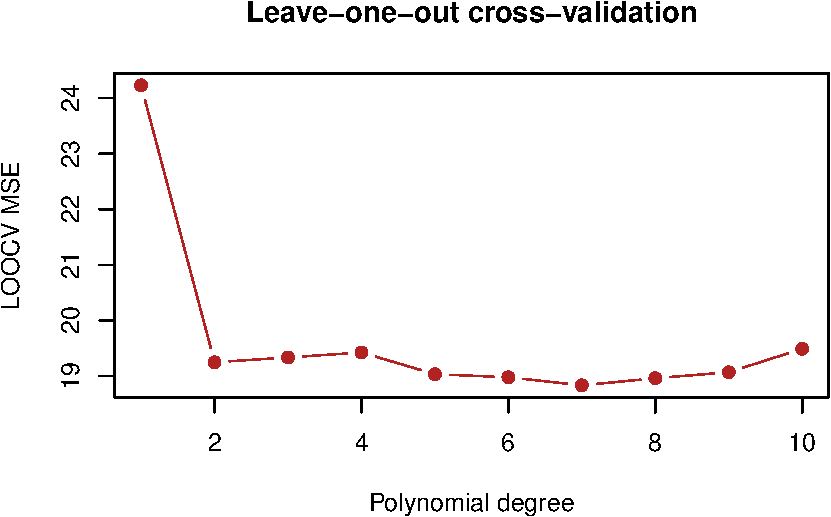
\includegraphics{ch05_lab_files/figure-latex/loocv-plot-1} \end{center}

The typical pattern is a large improvement from degree one to degree
two, followed by a flat curve. That means the quadratic term captures
important curvature, while higher-order terms do not produce a
dependable reduction in prediction error. LOOCV is attractive because
each fit uses almost the full data set, but it requires many model fits
and can be computationally costly for large data sets.

\section{\texorpdfstring{\(k\)-Fold
Cross-Validation}{k-Fold Cross-Validation}}\label{k-fold-cross-validation}

\subsection{Procedure and trade-off}\label{procedure-and-trade-off}

In \(k\)-fold cross-validation, the observations are divided into \(k\)
folds. Each fold is held out once while the other \(k-1\) folds are used
for training:

\[
\operatorname{CV}_{(k)}
= \frac{1}{k}\sum_{j=1}^{k}
\left(\frac{1}{|\mathcal{V}_j|}
\sum_{i\in\mathcal{V}_j}
\left(y_i-\hat{f}^{(-j)}(x_i)\right)^2\right).
\]

When \(k=n\), this becomes LOOCV. Common choices such as \(k=5\) or
\(k=10\) require far fewer fits while still using every observation for
validation. Smaller \(k\) can have slightly more bias because each
training set is smaller, but it is usually more computationally
efficient.

\begin{Shaded}
\begin{Highlighting}[]
\FunctionTok{set.seed}\NormalTok{(}\DecValTok{17}\NormalTok{)}
\NormalTok{kfold\_results }\OtherTok{\textless{}{-}} \FunctionTok{data.frame}\NormalTok{(}
  \AttributeTok{Degree =} \DecValTok{1}\SpecialCharTok{:}\DecValTok{10}\NormalTok{,}
  \AttributeTok{Tenfold\_CV\_MSE =} \ConstantTok{NA\_real\_}
\NormalTok{)}

\ControlFlowTok{for}\NormalTok{ (degree }\ControlFlowTok{in}\NormalTok{ kfold\_results}\SpecialCharTok{$}\NormalTok{Degree) \{}
\NormalTok{  model\_formula }\OtherTok{\textless{}{-}} \ControlFlowTok{if}\NormalTok{ (degree }\SpecialCharTok{==} \DecValTok{1}\NormalTok{) \{}
\NormalTok{    mpg }\SpecialCharTok{\textasciitilde{}}\NormalTok{ horsepower}
\NormalTok{  \} }\ControlFlowTok{else}\NormalTok{ \{}
\NormalTok{    mpg }\SpecialCharTok{\textasciitilde{}} \FunctionTok{poly}\NormalTok{(horsepower, degree)}
\NormalTok{  \}}
\NormalTok{  model }\OtherTok{\textless{}{-}} \FunctionTok{glm}\NormalTok{(model\_formula, }\AttributeTok{data =}\NormalTok{ Auto)}
\NormalTok{  kfold\_results}\SpecialCharTok{$}\NormalTok{Tenfold\_CV\_MSE[degree] }\OtherTok{\textless{}{-}}
    \FunctionTok{cv.glm}\NormalTok{(Auto, model, }\AttributeTok{K =} \DecValTok{10}\NormalTok{)}\SpecialCharTok{$}\NormalTok{delta[}\DecValTok{1}\NormalTok{]}
\NormalTok{\}}

\NormalTok{kfold\_results}
\end{Highlighting}
\end{Shaded}

\begin{verbatim}
##    Degree Tenfold_CV_MSE
## 1       1       24.27207
## 2       2       19.26909
## 3       3       19.34805
## 4       4       19.29496
## 5       5       19.03198
## 6       6       18.89781
## 7       7       19.12061
## 8       8       19.14666
## 9       9       18.87013
## 10     10       20.95520
\end{verbatim}

\begin{Shaded}
\begin{Highlighting}[]
\FunctionTok{plot}\NormalTok{(}
\NormalTok{  loocv\_results}\SpecialCharTok{$}\NormalTok{Degree, loocv\_results}\SpecialCharTok{$}\NormalTok{LOOCV\_MSE,}
  \AttributeTok{type =} \StringTok{"b"}\NormalTok{, }\AttributeTok{pch =} \DecValTok{19}\NormalTok{, }\AttributeTok{col =} \StringTok{"firebrick"}\NormalTok{,}
  \AttributeTok{xlab =} \StringTok{"Polynomial degree"}\NormalTok{, }\AttributeTok{ylab =} \StringTok{"Estimated test MSE"}\NormalTok{,}
  \AttributeTok{ylim =} \FunctionTok{range}\NormalTok{(}\FunctionTok{c}\NormalTok{(loocv\_results}\SpecialCharTok{$}\NormalTok{LOOCV\_MSE, kfold\_results}\SpecialCharTok{$}\NormalTok{Tenfold\_CV\_MSE)),}
  \AttributeTok{main =} \StringTok{"LOOCV and 10{-}fold CV"}
\NormalTok{)}
\FunctionTok{lines}\NormalTok{(}
\NormalTok{  kfold\_results}\SpecialCharTok{$}\NormalTok{Degree, kfold\_results}\SpecialCharTok{$}\NormalTok{Tenfold\_CV\_MSE,}
  \AttributeTok{type =} \StringTok{"b"}\NormalTok{, }\AttributeTok{pch =} \DecValTok{17}\NormalTok{, }\AttributeTok{col =} \StringTok{"steelblue"}
\NormalTok{)}
\FunctionTok{legend}\NormalTok{(}
  \StringTok{"topright"}\NormalTok{, }\AttributeTok{legend =} \FunctionTok{c}\NormalTok{(}\StringTok{"LOOCV"}\NormalTok{, }\StringTok{"10{-}fold CV"}\NormalTok{),}
  \AttributeTok{col =} \FunctionTok{c}\NormalTok{(}\StringTok{"firebrick"}\NormalTok{, }\StringTok{"steelblue"}\NormalTok{), }\AttributeTok{pch =} \FunctionTok{c}\NormalTok{(}\DecValTok{19}\NormalTok{, }\DecValTok{17}\NormalTok{), }\AttributeTok{lty =} \DecValTok{1}
\NormalTok{)}
\end{Highlighting}
\end{Shaded}

\begin{center}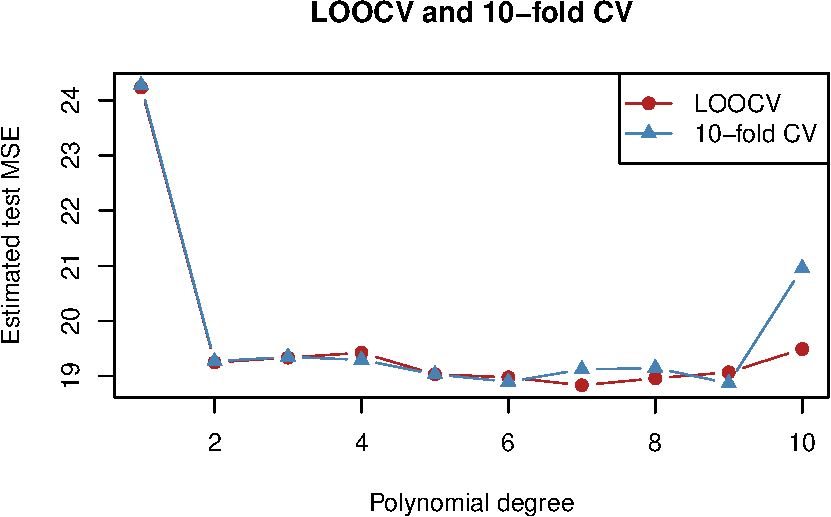
\includegraphics{ch05_lab_files/figure-latex/compare-cv-1} \end{center}

The two curves should have the same practical conclusion even though
their individual values differ slightly. Ten-fold CV is often the useful
default: it is much cheaper than LOOCV and generally gives a stable
estimate of the model's test error. Cross-validation estimates
prediction error; it does not prove that one model is the true
data-generating model.

\section{The Bootstrap}\label{the-bootstrap}

\subsection{The basic idea}\label{the-basic-idea}

Cross-validation focuses on prediction. The bootstrap focuses on
uncertainty in an estimate. We treat the observed sample as an
approximation to the population and repeatedly draw bootstrap samples of
size \(n\) \textbf{with replacement}. For a statistic
\(\hat{\theta}=T(Z_1,\ldots,Z_n)\), the \(b\)th bootstrap estimate is

\[
\hat{\theta}^{*b} = T(Z_1^{*b},\ldots,Z_n^{*b}),
\qquad b=1,\ldots,B.
\]

The standard deviation of the bootstrap estimates approximates the
standard error:

\[
\widehat{\operatorname{SE}}_{\mathrm{boot}}(\hat{\theta})
= \sqrt{\frac{1}{B-1}\sum_{b=1}^{B}
\left(\hat{\theta}^{*b}-\overline{\theta^*}\right)^2}.
\]

The phrase \emph{with replacement} is essential. It means some
observations may appear multiple times and some may be absent in a
particular bootstrap sample. That variation imitates the fact that a new
random sample would not contain exactly the same observations as the
original one.

\subsection{Portfolio allocation}\label{portfolio-allocation}

The \texttt{Portfolio} data set contains returns for two assets,
\texttt{X} and \texttt{Y}. Suppose we invest fraction \(\alpha\) in
asset \(X\) and \(1-\alpha\) in asset \(Y\). The portfolio return is

\[R_p = \alpha X + (1-\alpha)Y.\]

Minimizing its variance gives

\[
\hat{\alpha} =
\frac{\hat{\sigma}_Y^2-\hat{\sigma}_{XY}}
{\hat{\sigma}_X^2+\hat{\sigma}_Y^2-2\hat{\sigma}_{XY}}.
\]

This formula is easy to calculate on the original data. The uncertainty
in \(\hat{\alpha}\) is less obvious, so it is a good bootstrap example.

\begin{Shaded}
\begin{Highlighting}[]
\FunctionTok{data}\NormalTok{(Portfolio)}

\NormalTok{alpha\_function }\OtherTok{\textless{}{-}} \ControlFlowTok{function}\NormalTok{(data, index) \{}
\NormalTok{  X }\OtherTok{\textless{}{-}}\NormalTok{ data}\SpecialCharTok{$}\NormalTok{X[index]}
\NormalTok{  Y }\OtherTok{\textless{}{-}}\NormalTok{ data}\SpecialCharTok{$}\NormalTok{Y[index]}
\NormalTok{  (}\FunctionTok{var}\NormalTok{(Y) }\SpecialCharTok{{-}} \FunctionTok{cov}\NormalTok{(X, Y)) }\SpecialCharTok{/}
\NormalTok{    (}\FunctionTok{var}\NormalTok{(X) }\SpecialCharTok{+} \FunctionTok{var}\NormalTok{(Y) }\SpecialCharTok{{-}} \DecValTok{2} \SpecialCharTok{*} \FunctionTok{cov}\NormalTok{(X, Y))}
\NormalTok{\}}

\NormalTok{alpha\_hat }\OtherTok{\textless{}{-}} \FunctionTok{alpha\_function}\NormalTok{(Portfolio, }\FunctionTok{seq\_len}\NormalTok{(}\FunctionTok{nrow}\NormalTok{(Portfolio)))}

\FunctionTok{set.seed}\NormalTok{(}\DecValTok{7}\NormalTok{)}
\NormalTok{alpha\_boot }\OtherTok{\textless{}{-}} \FunctionTok{boot}\NormalTok{(Portfolio, alpha\_function, }\AttributeTok{R =} \DecValTok{1000}\NormalTok{)}
\NormalTok{alpha\_se }\OtherTok{\textless{}{-}} \FunctionTok{sd}\NormalTok{(alpha\_boot}\SpecialCharTok{$}\NormalTok{t)}
\NormalTok{alpha\_ci }\OtherTok{\textless{}{-}}\NormalTok{ alpha\_hat }\SpecialCharTok{+} \FunctionTok{c}\NormalTok{(}\SpecialCharTok{{-}}\DecValTok{1}\NormalTok{, }\DecValTok{1}\NormalTok{) }\SpecialCharTok{*} \FloatTok{1.96} \SpecialCharTok{*}\NormalTok{ alpha\_se}

\FunctionTok{data.frame}\NormalTok{(}
  \AttributeTok{Estimate =}\NormalTok{ alpha\_hat,}
  \AttributeTok{Bootstrap\_SE =}\NormalTok{ alpha\_se,}
  \AttributeTok{CI\_lower =}\NormalTok{ alpha\_ci[}\DecValTok{1}\NormalTok{],}
  \AttributeTok{CI\_upper =}\NormalTok{ alpha\_ci[}\DecValTok{2}\NormalTok{]}
\NormalTok{)}
\end{Highlighting}
\end{Shaded}

\begin{verbatim}
##    Estimate Bootstrap_SE  CI_lower  CI_upper
## 1 0.5758321   0.08978204 0.3998593 0.7518049
\end{verbatim}

The estimate is the suggested fraction invested in asset \(X\),
conditional on the observed sample. The bootstrap standard error says
how much this allocation would typically move across comparable samples.
The approximate normal-theory interval is computed as

\[
\hat{\alpha} \pm 1.96\,\widehat{\operatorname{SE}}_{\mathrm{boot}}.
\]

This interval is an uncertainty statement, not a guarantee that future
returns will lie inside it. It describes uncertainty in the estimated
allocation, while the investment decision itself also requires a risk
model and practical constraints.

\begin{Shaded}
\begin{Highlighting}[]
\FunctionTok{hist}\NormalTok{(}
\NormalTok{  alpha\_boot}\SpecialCharTok{$}\NormalTok{t, }\AttributeTok{breaks =} \DecValTok{30}\NormalTok{, }\AttributeTok{col =} \StringTok{"grey85"}\NormalTok{, }\AttributeTok{border =} \StringTok{"white"}\NormalTok{,}
  \AttributeTok{xlab =} \FunctionTok{expression}\NormalTok{(alpha}\SpecialCharTok{\^{}}\StringTok{"*"}\NormalTok{),}
  \AttributeTok{main =} \StringTok{"Bootstrap distribution of the portfolio weight"}
\NormalTok{)}
\FunctionTok{abline}\NormalTok{(}\AttributeTok{v =}\NormalTok{ alpha\_hat, }\AttributeTok{col =} \StringTok{"firebrick"}\NormalTok{, }\AttributeTok{lwd =} \DecValTok{2}\NormalTok{)}
\FunctionTok{abline}\NormalTok{(}\AttributeTok{v =}\NormalTok{ alpha\_ci, }\AttributeTok{col =} \StringTok{"steelblue"}\NormalTok{, }\AttributeTok{lty =} \DecValTok{2}\NormalTok{, }\AttributeTok{lwd =} \DecValTok{2}\NormalTok{)}
\FunctionTok{legend}\NormalTok{(}
  \StringTok{"topright"}\NormalTok{,}
  \AttributeTok{legend =} \FunctionTok{c}\NormalTok{(}\StringTok{"Original estimate"}\NormalTok{, }\StringTok{"Approx. 95\% interval"}\NormalTok{),}
  \AttributeTok{col =} \FunctionTok{c}\NormalTok{(}\StringTok{"firebrick"}\NormalTok{, }\StringTok{"steelblue"}\NormalTok{), }\AttributeTok{lty =} \FunctionTok{c}\NormalTok{(}\DecValTok{1}\NormalTok{, }\DecValTok{2}\NormalTok{), }\AttributeTok{lwd =} \DecValTok{2}
\NormalTok{)}
\end{Highlighting}
\end{Shaded}

\begin{center}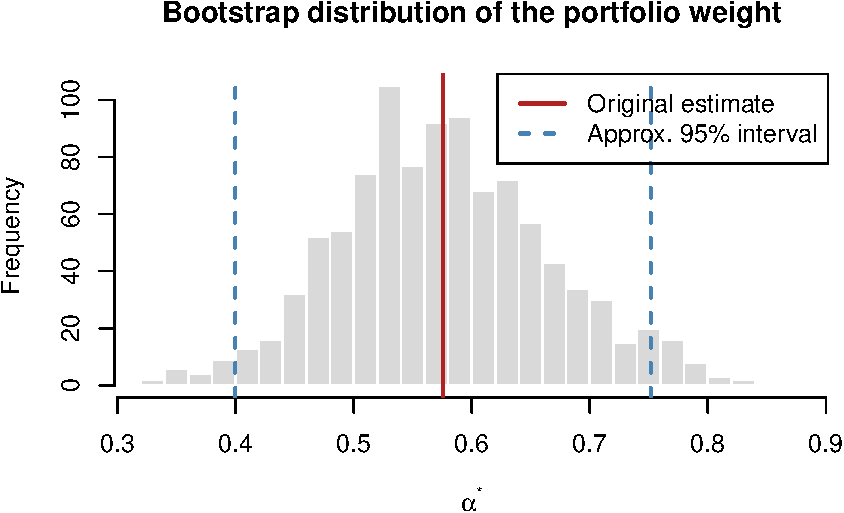
\includegraphics{ch05_lab_files/figure-latex/portfolio-bootstrap-plot-1} \end{center}

\subsection{Bootstrap standard errors for regression
coefficients}\label{bootstrap-standard-errors-for-regression-coefficients}

The bootstrap can estimate uncertainty for almost any statistic that can
be computed from a data set. Here the statistic is the vector of
coefficients from a regression of \texttt{mpg} on \texttt{horsepower}.

\begin{Shaded}
\begin{Highlighting}[]
\NormalTok{coefficient\_function }\OtherTok{\textless{}{-}} \ControlFlowTok{function}\NormalTok{(data, index) \{}
  \FunctionTok{coef}\NormalTok{(}\FunctionTok{lm}\NormalTok{(mpg }\SpecialCharTok{\textasciitilde{}}\NormalTok{ horsepower, }\AttributeTok{data =}\NormalTok{ data, }\AttributeTok{subset =}\NormalTok{ index))}
\NormalTok{\}}

\NormalTok{coefficient\_hat }\OtherTok{\textless{}{-}} \FunctionTok{coefficient\_function}\NormalTok{(Auto, }\FunctionTok{seq\_len}\NormalTok{(}\FunctionTok{nrow}\NormalTok{(Auto)))}

\FunctionTok{set.seed}\NormalTok{(}\DecValTok{1}\NormalTok{)}
\NormalTok{coefficient\_boot }\OtherTok{\textless{}{-}} \FunctionTok{boot}\NormalTok{(Auto, coefficient\_function, }\AttributeTok{R =} \DecValTok{1000}\NormalTok{)}

\NormalTok{coefficient\_summary }\OtherTok{\textless{}{-}} \FunctionTok{data.frame}\NormalTok{(}
  \AttributeTok{Term =} \FunctionTok{names}\NormalTok{(coefficient\_hat),}
  \AttributeTok{Estimate =} \FunctionTok{unname}\NormalTok{(coefficient\_hat),}
  \AttributeTok{Bootstrap\_SE =} \FunctionTok{apply}\NormalTok{(coefficient\_boot}\SpecialCharTok{$}\NormalTok{t, }\DecValTok{2}\NormalTok{, sd),}
  \AttributeTok{Classical\_SE =} \FunctionTok{coef}\NormalTok{(}\FunctionTok{summary}\NormalTok{(}\FunctionTok{lm}\NormalTok{(mpg }\SpecialCharTok{\textasciitilde{}}\NormalTok{ horsepower, }\AttributeTok{data =}\NormalTok{ Auto)))[, }\StringTok{"Std. Error"}\NormalTok{]}
\NormalTok{)}
\NormalTok{coefficient\_summary}
\end{Highlighting}
\end{Shaded}

\begin{verbatim}
##                    Term   Estimate Bootstrap_SE Classical_SE
## (Intercept) (Intercept) 39.9358610  0.843931305  0.717498656
## horsepower   horsepower -0.1578447  0.007367396  0.006445501
\end{verbatim}

The slope is negative: cars with greater horsepower tend to have lower
fuel efficiency. The bootstrap standard error measures the variability
of that slope under repeated samples. Comparing it with the usual
regression standard error is a useful diagnostic. Similar values suggest
that the classical approximation is reasonable here; noticeable
differences remind us that standard errors depend on assumptions about
the model and its errors.

We can also bootstrap a nonlinear specification. The quadratic
coefficient measures curvature, so its uncertainty helps us decide
whether the observed curvature is stable enough to support the added
model complexity.

\begin{Shaded}
\begin{Highlighting}[]
\NormalTok{quadratic\_function }\OtherTok{\textless{}{-}} \ControlFlowTok{function}\NormalTok{(data, index) \{}
  \FunctionTok{coef}\NormalTok{(}\FunctionTok{lm}\NormalTok{(mpg }\SpecialCharTok{\textasciitilde{}}\NormalTok{ horsepower }\SpecialCharTok{+} \FunctionTok{I}\NormalTok{(horsepower}\SpecialCharTok{\^{}}\DecValTok{2}\NormalTok{),}
          \AttributeTok{data =}\NormalTok{ data, }\AttributeTok{subset =}\NormalTok{ index))}
\NormalTok{\}}

\FunctionTok{set.seed}\NormalTok{(}\DecValTok{1}\NormalTok{)}
\NormalTok{quadratic\_boot }\OtherTok{\textless{}{-}} \FunctionTok{boot}\NormalTok{(Auto, quadratic\_function, }\AttributeTok{R =} \DecValTok{1000}\NormalTok{)}

\FunctionTok{data.frame}\NormalTok{(}
  \AttributeTok{Term =} \FunctionTok{names}\NormalTok{(}\FunctionTok{coef}\NormalTok{(}\FunctionTok{lm}\NormalTok{(mpg }\SpecialCharTok{\textasciitilde{}}\NormalTok{ horsepower }\SpecialCharTok{+} \FunctionTok{I}\NormalTok{(horsepower}\SpecialCharTok{\^{}}\DecValTok{2}\NormalTok{), }\AttributeTok{data =}\NormalTok{ Auto))),}
  \AttributeTok{Estimate =} \FunctionTok{coef}\NormalTok{(}\FunctionTok{lm}\NormalTok{(mpg }\SpecialCharTok{\textasciitilde{}}\NormalTok{ horsepower }\SpecialCharTok{+} \FunctionTok{I}\NormalTok{(horsepower}\SpecialCharTok{\^{}}\DecValTok{2}\NormalTok{), }\AttributeTok{data =}\NormalTok{ Auto)),}
  \AttributeTok{Bootstrap\_SE =} \FunctionTok{apply}\NormalTok{(quadratic\_boot}\SpecialCharTok{$}\NormalTok{t, }\DecValTok{2}\NormalTok{, sd)}
\NormalTok{)}
\end{Highlighting}
\end{Shaded}

\begin{verbatim}
##                            Term     Estimate Bootstrap_SE
## (Intercept)         (Intercept) 56.900099702 2.0300222526
## horsepower           horsepower -0.466189630 0.0324241984
## I(horsepower^2) I(horsepower^2)  0.001230536 0.0001172164
\end{verbatim}

\section{Putting the Methods
Together}\label{putting-the-methods-together}

The methods answer different questions, so their outputs should not be
confused:

{\def\LTcaptype{none} % do not increment counter
\begin{longtable}[]{@{}
  >{\raggedright\arraybackslash}p{(\linewidth - 4\tabcolsep) * \real{0.3333}}
  >{\raggedright\arraybackslash}p{(\linewidth - 4\tabcolsep) * \real{0.3333}}
  >{\raggedright\arraybackslash}p{(\linewidth - 4\tabcolsep) * \real{0.3333}}@{}}
\toprule\noalign{}
\begin{minipage}[b]{\linewidth}\raggedright
Method
\end{minipage} & \begin{minipage}[b]{\linewidth}\raggedright
Main question
\end{minipage} & \begin{minipage}[b]{\linewidth}\raggedright
Mechanism
\end{minipage} \\
\midrule\noalign{}
\endhead
\bottomrule\noalign{}
\endlastfoot
Validation set & How well does this model predict on one held-out split?
& One train/validation split \\
LOOCV & What is the average held-out error when each observation is left
out? & \(n\) fits \\
\(k\)-fold CV & What is held-out error using a practical number of
folds? & \(k\) fits \\
Bootstrap & How variable is an estimate across plausible samples? &
Resample with replacement \\
\end{longtable}
}

For the \texttt{Auto} analysis, the resampling results generally support
a quadratic relationship between \texttt{mpg} and \texttt{horsepower}:
degree two improves on degree one, while higher degrees provide little
dependable improvement. This is a model-selection conclusion about
predictive performance, not a claim that a quadratic law is physically
exact.

The broader lesson is that a fitted model is only one estimate obtained
from one sample. Validation and cross-validation expose how prediction
changes when observations are held out. The bootstrap exposes how
statistical summaries change when the observed sample is perturbed.
Together they provide an empirical way to reason about generalization
and uncertainty rather than reporting training fit alone.

\section{Conclusion}\label{conclusion}

Resampling methods turn a single data set into a collection of
informative experiments. The validation set is simple but unstable.
LOOCV uses data efficiently but can be expensive. Ten-fold
cross-validation is often a good practical compromise for comparing
model complexity. The bootstrap is more general: it estimates standard
errors for statistics whose sampling distributions are difficult to
derive analytically.

The most important habit is to match the resampling method to the
question. Use held-out predictions when the concern is generalization,
and use bootstrap replicates when the concern is the uncertainty of an
estimate. Neither method removes irreducible noise, but both make the
limits of what we learn from a finite sample much more visible.

\end{document}
